\documentclass[12pt]{article}
\usepackage{tikz}
\usetikzlibrary{arrows.meta}

\begin{document}

\section{Nodes}

\subsection{Scaled Node}
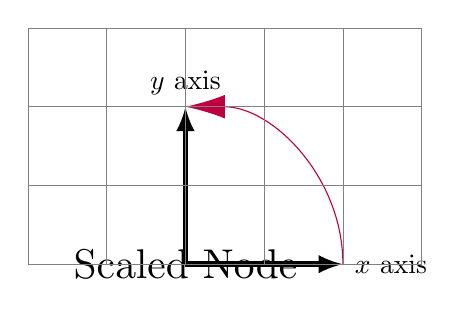
\begin{tikzpicture}[xscale=1]
      \coordinate (O) at (0,0);
      \node[scale=1.5] at (O) {Scaled Node};
      \draw[line width=2, -latex] (O)--(2,0) node[right] {$x$ axis};
      \draw[line width=2, -latex] (O)--(0,2) node[above] {$y$ axis};
      \draw[-{Latex[length=5mm, width=3mm]}, purple] (2,0) arc (0:90:2);
      \draw[step=1cm, gray, very thin] (-2,0) grid (3,3);
\end{tikzpicture}

\subsection{Rotated Node}
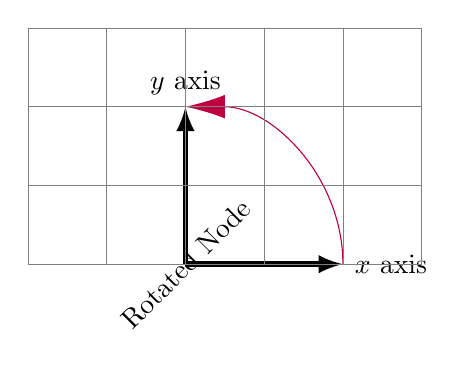
\begin{tikzpicture}[xscale=1]
      \coordinate (O) at (0,0);
      \node[rotate=45] at (O) {Rotated Node};
      \draw[line width=2, -latex] (O)--(2,0) node[right] {$x$ axis};
      \draw[line width=2, -latex] (O)--(0,2) node[above] {$y$ axis};
      \draw[-{Latex[length=5mm, width=3mm]}, purple] (2,0) arc (0:90:2);
      \draw[step=1cm, gray, very thin] (-2,0) grid (3,3);
\end{tikzpicture}

\subsection{Below Node}
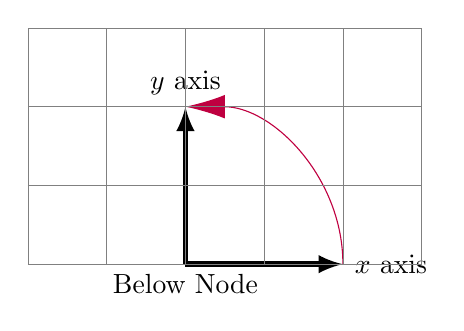
\begin{tikzpicture}[xscale=1]
      \coordinate (O) at (0,0);
      \node[below] at (O) {Below Node};
      \draw[line width=2, -latex] (O)--(2,0) node[right] {$x$ axis};
      \draw[line width=2, -latex] (O)--(0,2) node[above] {$y$ axis};
      \draw[-{Latex[length=5mm, width=3mm]}, purple] (2,0) arc (0:90:2);
      \draw[step=1cm, gray, very thin] (-2,0) grid (3,3);
\end{tikzpicture}

\subsection{Above Node}
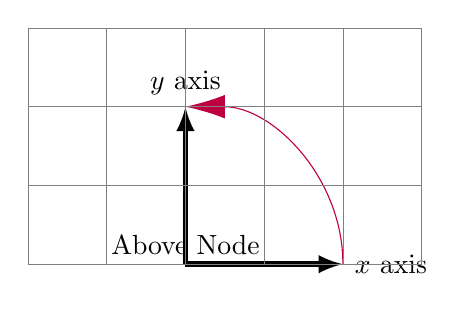
\begin{tikzpicture}[xscale=1]
      \coordinate (O) at (0,0);
      \node[above] at (O) {Above Node};
      \draw[line width=2, -latex] (O)--(2,0) node[right] {$x$ axis};
      \draw[line width=2, -latex] (O)--(0,2) node[above] {$y$ axis};
      \draw[-{Latex[length=5mm, width=3mm]}, purple] (2,0) arc (0:90:2);
      \draw[step=1cm, gray, very thin] (-2,0) grid (3,3);
\end{tikzpicture}

\subsection{Above Node}
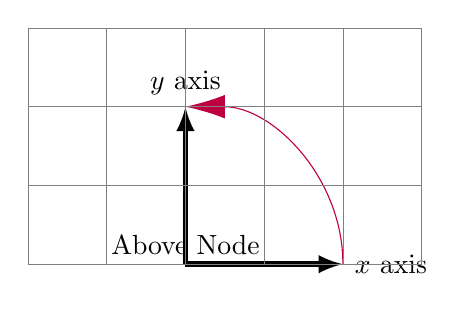
\begin{tikzpicture}[xscale=1]
      \coordinate (O) at (0,0);
      \node[above] at (O) {Above Node};
      \draw[line width=2, -latex] (O)--(2,0) node[right] {$x$ axis};
      \draw[line width=2, -latex] (O)--(0,2) node[above] {$y$ axis};
      \draw[-{Latex[length=5mm, width=3mm]}, purple] (2,0) arc (0:90:2);
      \draw[step=1cm, gray, very thin] (-2,0) grid (3,3);
\end{tikzpicture}

\subsection{Left Node}
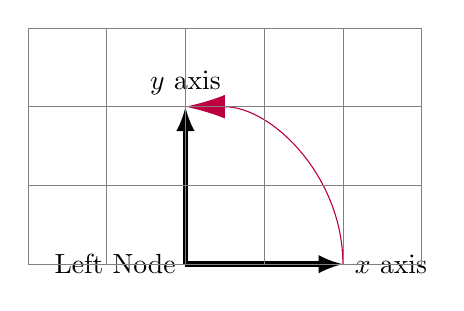
\begin{tikzpicture}[xscale=1]
      \coordinate (O) at (0,0);
      \node[left] at (O) {Left Node};
      \draw[line width=2, -latex] (O)--(2,0) node[right] {$x$ axis};
      \draw[line width=2, -latex] (O)--(0,2) node[above] {$y$ axis};
      \draw[-{Latex[length=5mm, width=3mm]}, purple] (2,0) arc (0:90:2);
      \draw[step=1cm, gray, very thin] (-2,0) grid (3,3);
\end{tikzpicture}

\subsection{Right Node}
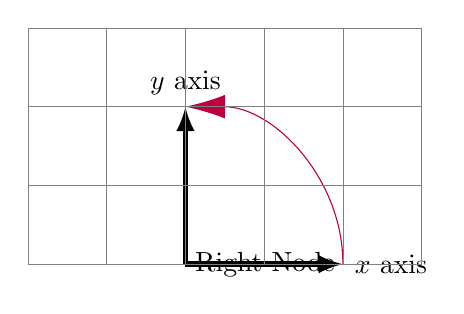
\begin{tikzpicture}[xscale=1]
      \coordinate (O) at (0,0);
      \node[right] at (O) {Right Node};
      \draw[line width=2, -latex] (O)--(2,0) node[right] {$x$ axis};
      \draw[line width=2, -latex] (O)--(0,2) node[above] {$y$ axis};
      \draw[-{Latex[length=5mm, width=3mm]}, purple] (2,0) arc (0:90:2);
      \draw[step=1cm, gray, very thin] (-2,0) grid (3,3);
\end{tikzpicture}

\subsection{Below Left Node}
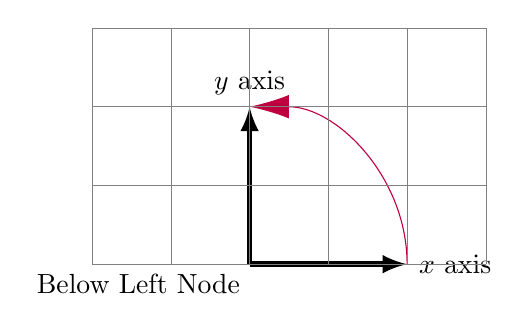
\begin{tikzpicture}[xscale=1]
      \coordinate (O) at (0,0);
      \node[below left] at (O) {Below Left Node};
      \draw[line width=2, -latex] (O)--(2,0) node[right] {$x$ axis};
      \draw[line width=2, -latex] (O)--(0,2) node[above] {$y$ axis};
      \draw[-{Latex[length=5mm, width=3mm]}, purple] (2,0) arc (0:90:2);
      \draw[step=1cm, gray, very thin] (-2,0) grid (3,3);
\end{tikzpicture}

\subsection{Below Right Node}
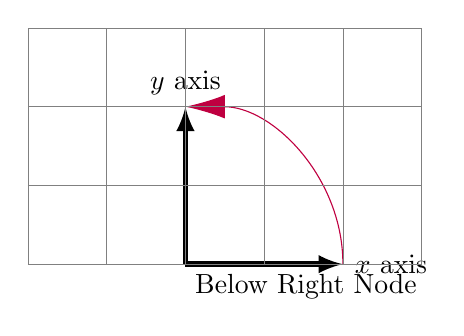
\begin{tikzpicture}[xscale=1]
      \coordinate (O) at (0,0);
      \node[below right] at (O) {Below Right Node};
      \draw[line width=2, -latex] (O)--(2,0) node[right] {$x$ axis};
      \draw[line width=2, -latex] (O)--(0,2) node[above] {$y$ axis};
      \draw[-{Latex[length=5mm, width=3mm]}, purple] (2,0) arc (0:90:2);
      \draw[step=1cm, gray, very thin] (-2,0) grid (3,3);
\end{tikzpicture}

\subsection{Above Right Node}
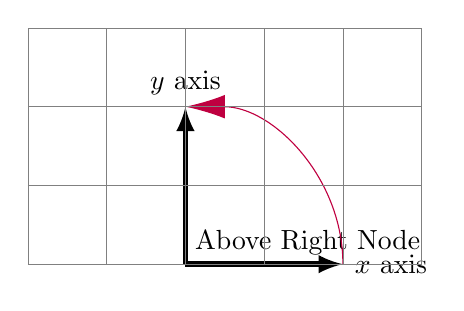
\begin{tikzpicture}[xscale=1]
      \coordinate (O) at (0,0);
      \node[above right] at (O) {Above Right Node};
      \draw[line width=2, -latex] (O)--(2,0) node[right] {$x$ axis};
      \draw[line width=2, -latex] (O)--(0,2) node[above] {$y$ axis};
      \draw[-{Latex[length=5mm, width=3mm]}, purple] (2,0) arc (0:90:2);
      \draw[step=1cm, gray, very thin] (-2,0) grid (3,3);
\end{tikzpicture}

\subsection{Above Left Node}
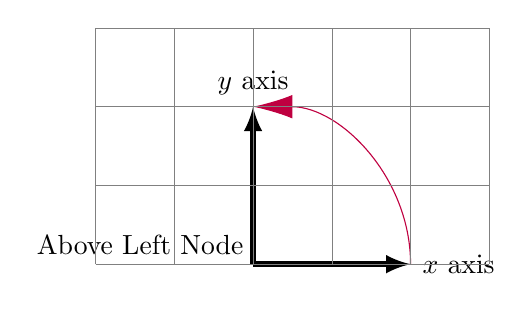
\begin{tikzpicture}[xscale=1]
      \coordinate (O) at (0,0);
      \node[above left] at (O) {Above Left Node};
      \draw[line width=2, -latex] (O)--(2,0) node[right] {$x$ axis};
      \draw[line width=2, -latex] (O)--(0,2) node[above] {$y$ axis};
      \draw[-{Latex[length=5mm, width=3mm]}, purple] (2,0) arc (0:90:2);
      \draw[step=1cm, gray, very thin] (-2,0) grid (3,3);
\end{tikzpicture}

\subsection{xshift Node}
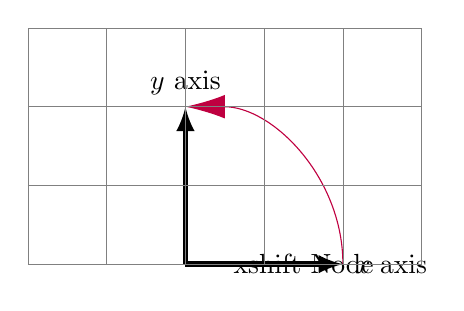
\begin{tikzpicture}[xscale=1]
      \coordinate (O) at (0,0);
      \node[xshift=1.5cm] at (O) {xshift Node};
      \draw[line width=2, -latex] (O)--(2,0) node[right] {$x$ axis};
      \draw[line width=2, -latex] (O)--(0,2) node[above] {$y$ axis};
      \draw[-{Latex[length=5mm, width=3mm]}, purple] (2,0) arc (0:90:2);
      \draw[step=1cm, gray, very thin] (-2,0) grid (3,3);
\end{tikzpicture}

\subsection{yshift Node}
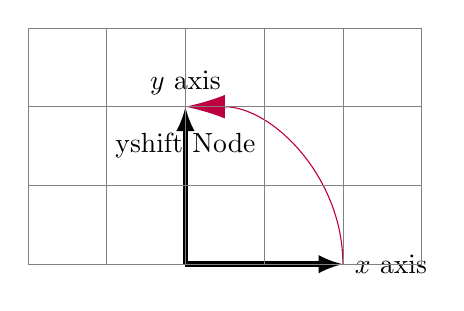
\begin{tikzpicture}[xscale=1]
      \coordinate (O) at (0,0);
      \node[yshift=1.5cm] at (O) {yshift Node};
      \draw[line width=2, -latex] (O)--(2,0) node[right] {$x$ axis};
      \draw[line width=2, -latex] (O)--(0,2) node[above] {$y$ axis};
      \draw[-{Latex[length=5mm, width=3mm]}, purple] (2,0) arc (0:90:2);
      \draw[step=1cm, gray, very thin] (-2,0) grid (3,3);
\end{tikzpicture}

\end{document}
